%!TeX root=../tese.tex
%("dica" para o editor de texto: este arquivo é parte de um documento maior)
% para saber mais: https://tex.stackexchange.com/q/78101

%% ------------------------------------------------------------------------- %%

% "\chapter" cria um capítulo com número e o coloca no sumário; "\chapter*"
% cria um capítulo sem número e não o coloca no sumário. A introdução não
% deve ser numerada, mas deve aparecer no sumário. Por conta disso, este
% modelo define o comando "\unnumberedchapter".
\unnumberedchapter{Introduction}
\label{cap:introducao}

\enlargethispage{.5\baselineskip}

As defined by \citet{matsakis2014rust} the Rust programming language is a modern
systems programming language focused on safety, speed and concurrency. It compares
to C++ in terms of mapping directly to hardware, but it is safer to use thanks to
the guarantees it's static type system provides. The language has been successfully
used on a number of different domains, including astrophysics \citep{blanco2016can}
and operating system kernels development \citep{levy2017case}.

The Rust compiler is a complex piece of software, with many different components.
It is written in Rust itself, making it a self-hosted language, and it is composed
of a Rust front-end, a LLVM middle-end and a LLVM back-end.

As described by the \citet{rustc-dev-guide} the front-end is responsible for parsing
the source code, desugaring, checking and validating it, and generating a first intermediate
representation of the code, called High-level Intermediate Representation (HIR).
After this, the middle-end is responsible for lowering the HIR to a lower-level representation
called Middle-level Intermediate Representation (MIR) by doing type checking. On the next step,
the compiler enforces the borrow checking rules, which are one of the main features of the Rust language,
and executes some initial optimizations, finally lowering the MIR to an IR called LLVM IR. From here on,
the LLVM middle-end enters and starts to transform the LLVM IR into a more optimized version of itself.
Finally, the LLVM back-end is responsible for lowering the LLVM IR to the target machine assembly code. It's important
to notice that the Rust compiler is not tied to the LLVM compiler framework, but it is the most used back-end.
A high-level overview of the Rust compilation pipeline can be seen on Figure~\ref{fig:rustc-pipeline}.

\begin{figure}[ht]
    \centering
    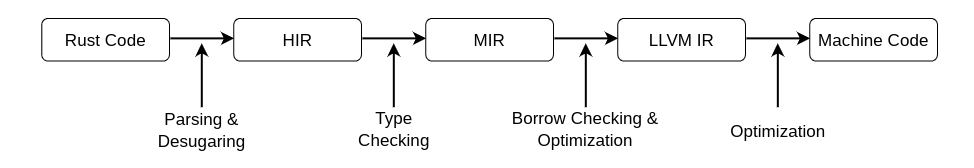
\includegraphics[width=1\textwidth]{figuras/rustc.png}
    \caption{Overview of the Rust compilation pipeline}
    \label{fig:rustc-pipeline}
\end{figure}


%% ------------------------------------------------------------------------- %%
\unnumberedsection{LLVM Optimizations}
\label{sec:consideracoes_preliminares}

Normalmente, as citações não devem fazer parte da estrutura sintática da
frase\footnote{E não se deve abusar das notas de rodapé.\index{Notas de rodapé}}.
No entanto, usando referências em algum estilo autor-data (como o estilo
plainnat do \LaTeX{}), é comum que o nome do autor faça parte da frase. Nesses
casos, pode valer a pena mudar o formato da citação para não repetir o nome do
autor; no \LaTeX{}, isso pode ser feito usando os comandos
\textsf{\textbackslash{}citet}, \textsf{\textbackslash{}citep},
\textsf{\textbackslash{}citeyear} etc. documentados no pacote
natbib \citep{natbib}\index{natbib} (esses comandos são compatíveis com biblatex
usando a opção \textsf{natbib=true}, ativada por padrão neste modelo). Em geral,
portanto, as citações devem seguir estes exemplos:

\footnotesize
\begin{verbatim}
Modos de citação:
indesejável: [AF83] introduziu o algoritmo ótimo.
indesejável: (Andrew e Foster, 1983) introduziram o algoritmo ótimo.
certo: Andrew e Foster introduziram o algoritmo ótimo [AF83].
certo: Andrew e Foster introduziram o algoritmo ótimo (Andrew e Foster, 1983).
certo (\citet ou \citeyear): Andrew e Foster (1983) introduziram o algoritmo ótimo.
\end{verbatim}
\normalsize

\enlargethispage{.5\baselineskip}

O uso desnecessário de termos em língua estrangeira deve ser evitado. No entanto,
quando isso for necessário, os termos devem aparecer \textit{em itálico}.
\index{Língua estrangeira}
% index permite acrescentar um item no indice remissivo

Uma prática recomendável na escrita de textos é descrever as
legendas\index{Legendas} das figuras e tabelas em forma auto-contida: as
legendas devem ser razoavelmente completas, de modo que o leitor possa entender
a figura sem ler o texto em que a figura ou tabela é citada.\index{Floats}

\unnumberedsection{Ferramentas bibliográficas}

Embora seja possível pesquisar por material acadêmico na Internet usando
sistemas de busca ``comuns'', existem ferramentas dedicadas, como o
\textsf{Google Scholar}\index{Google Scholar} (\url{scholar.google.com}).
O \textsf{Web of Science}\index{Web of Science}
(\url{webofscience.com}) e o \textsf{Scopus}\index{Scopus} (\url{scopus.com})
oferecem recursos sofisticados e limitam a busca a periódicos com boa
reputação acadêmica. Essas duas plataformas não são gratuitas, mas os alunos
da USP têm acesso a elas através da instituição. Algumas editoras, como a
ACM (\url{dl.acm.org}) e a IEEE (\url{ieeexplore.ieee.org}), também têm
sistemas de busca bibliográfica. Todas essas ferramentas são capazes de
exportar os dados para o formato .bib, usado pelo \LaTeX{} (no Google
Scholar, é preciso ativar a opção correspondente nas preferências). O sítio
\url{liinwww.ira.uka.de/bibliography} também permite buscar e baixar
referências bibliográficas relevantes para a área de computação.

Lamentavelmente, ainda não existe um mecanismo de verificação ou validação
das informações nessas plataformas. Portanto, é fortemente sugerido validar
todas as informações de tal forma que as entradas bib estejam corretas.
De qualquer modo, tome muito cuidado na padronização das referências
bibliográficas: ou considere TODOS os nomes dos autores por extenso, ou
TODOS os nomes dos autores abreviados. Evite misturas inapropriadas.\looseness=-1

Apenas uma parte dos artigos acadêmicos de interesse está disponível livremente
na Internet; os demais são restritos a assinantes. A CAPES assina um grande
volume de publicações e disponibiliza o acesso a elas para diversas universidades
brasileiras, entre elas a USP, através do seu portal de periódicos
(\url{periodicos.capes.gov.br}). Existe uma extensão para os navegadores
Chrome e Firefox (\url{www.infis.ufu.br/capes-periodicos}) que facilita o uso
cotidiano do portal.

Para manter um banco de dados organizado sobre artigos e outras fontes bibliográficas
relevantes para sua pesquisa, é altamente recomendável que você use uma ferramenta
como Zotero~(\url{zotero.org})\index{Zotero} ou
Mendeley~(\url{mendeley.com})\index{Mendeley}. Ambas podem exportar seus dados no
formato .bib, compatível com \LaTeX{}.
